\documentclass[12pt]{article}

\usepackage[T1]{fontenc}
\usepackage[margin=1in]{geometry}
\usepackage{amsmath}
\usepackage{graphicx}
\usepackage{algorithm}
\usepackage{algpseudocode}
\usepackage{caption}

\title{
	\textbf{Assignment 05\\}
		Solving Boundary Value Problem\\
		Using Finite Difference Method
}
\author{Mayank Pathania\\204103314}
\date{\today}

\begin{document}
	\maketitle
	
	\section{Formulation}
    Boundary value problem is of the form
	\[x^{''} = f(t,x,x^{'}) \]
    \[in\;a\leq t \leq b \; with \; x(a)=\alpha;\; x(b)=\beta\]
	\textbf{Central difference formula:}
    \[x^{'}(t)=\frac{1}{2h}[x(t+h) - x(t - h)]\]
    \[x^{''}(t)=\frac{1}{h^2}[x(t+h)-2x(t)+x(t-h)]\]
    where h is spacing between consecutive data points. For equal spacing \[h = (\frac{b -a}{n})\] where n is number of intervals.\\
    \textbf{Given Problem:}
    \[x^{''} = xsin(t) + x^{'}cos(t)-e^{t}\]
    \[x(0) = 0;\; x(1) = 1;\]
    The problem can be written using central difference formulas as
    \[\frac{1}{h^2}[x(t + h) - 2x(t) + x(t - h)] = x_isin(t_i) + \frac{1}{2h}[x(t + h) - x(t - h)]cos(t_i) - e^{t_i}\]
    \[\frac{1}{h^2}(x_{i+1}-2x_i+x_{i-1}) = x_isin(t_i) + \frac{1}{2h}(x_{i+1} - x_{i-1})cos(t_i) - e^{t_i}\]
    where \[t_i = a + ih\;\;\;\;i = 1,\;2,....,n-1\] \[x_{i}=x(t_i)\]
    now collecting $x_{i+1},\;x_i,\;x_{i-1}$ terms on LHS and terms without $x$ on RHS we get
    \[(\frac{1}{h^2} - \frac{cos(t_i)}{2h})x_{i+1} -(\frac{2}{h^2} + sin(t_i))x_i + (\frac{1}{h^2} + \frac{cos(t_i)}{2h})x_{i-1} = -e^{t_i}\]
    multiplying both side by $h^2$ we get
    \[(1 - \frac{hcos(t_i)}{2})x_{i+1} -(2 + h^{2}sin(t_i))x_i + (1 + \frac{hcos(t_i)}{2})x_{i-1} = -h^{2}e^{t_i}\]
    Then we can write this above equation in the form 
    \[a_ix_{i-1} + d_ix_{i} + c_ix_{i + 1} = b_i\]
    where \[a_i = (1 + \frac{hcos(t_i)}{2})\]
        \[b_i = -h^{2}e^{t_i}\]
        \[d_i = -(2 + h^{2}sin(t_i))\]
        \[c_i = (1 - \frac{hcos(t_i)}{2})\]
    as $x_0 = \alpha$ and $x_n = \beta$ are known we can write the above equation as
    \[d_1x_{1} + c_1x_{2} = b_1 - a_1\alpha\]
    \[a_2x_{1} + d_2x_{2} + c_2x_{3} = b_2\]
    \[a_3x_{2} + d_3x_{3} + c_3x_{4} = b_3\]
    \[\vdots\;\;\vdots\]
    \[a_{n - 1}x_{n - 2} + d_{n - 1}x_{n - 1} = b_{n - 1} - c_{n - 1}\beta\]
    Now these equations can be written in matrix form as
    \begin{center}$
        \begin{bmatrix}
            d_1 & c_1\ & 0 & 0 & 0 & ... & 0 & 0\\
            a_2 & d_2 & c_2 & 0 & 0 & ... & 0 & 0\\
            0 & a_3 & d_3 & c_3 & 0 & ... & 0 & 0 \\
            \vdots & \vdots & \vdots & \vdots & \vdots & \hdots & 0 & 0\\
            0 & 0 & 0 & 0 & 0 & \hdots & a_{n - 1} & d_{n - 1}\\
        \end{bmatrix}
        \begin{Bmatrix}
            x_1\\
            x_2\\
            x_3\\
            \vdots\\
            x_{n - 1}
        \end{Bmatrix}
        =
        \begin{Bmatrix}
            b_1 - a_1\alpha\\
            b_2\\
            b_3\\
            \vdots\\
            b_{n - 1} - c_{n - 1}\beta
        \end{Bmatrix}
        $
    \end{center}
    The matrix is tridiagonal matrix. And the problem is of the form \textbf{Ax = B} and it can be solved using gauss elimination method.

    \pagebreak
	\section{Algorithms}
	\subsection{Initialization}
	\begin{center}
		\begin{algorithmic}[1]
			\Procedure{fill\_AB}{m, a, b, $\alpha$, $\beta$}
			\Statex \Comment{m = number of intervals - 1}
			\Statex \Comment{x(a) = $\alpha$; x(b) = $\beta$}
			\State A $\gets$ initialize matriz of size m$\times$3 \Comment{Only tridiagonal elements are stored}
			\State B $\gets$ initialize vector of size m
			\For{i$\gets$1:1:m}
			\State \Comment{$a_i, b_i, c_i, d_i$ are from formulation}
			\If{i > 1}
			\State A[i][1] $\gets$ $a_i$
			\EndIf
			\State A[i][2] $\gets$ $d_i$
			\If{i < m}
			\State A[i][3] $\gets$ $c_i$
			\EndIf
			\State B[i] $\gets$ $b_i$
			\EndFor
			\State B[0] $\gets$ B[0] - $a_1*\alpha$
			\State B[m] $\gets$ B[m] - $c_{m}*\beta$
            \State \textbf{return} A,B
			\EndProcedure
		\end{algorithmic}
	\end{center}

    \subsection{Solving Ax = B}
    \begin{center}
        \begin{algorithmic}[1]
            \Procedure{solve}{A[][], B[]}
                \Statex \Comment{A[][] is matrix of size m $\times$ 3}
                \Statex \Comment{B[] is vector of size m $\times$ 1}
                \Statex \Comment{Elimination Steps}
                \For{i$\gets$1:1:m-1}
                    \State ratio $\gets \;\frac{A[i + 1][1]}{A[i][2]}$
                    \State A[i + 1][2] $\gets$ A[i + 1][2] - (ratio $\times$ A[i][3])
                    \State B[i + 1] $\gets$ B[i + 1] - (ratio $\times$ B[i]) 
                \EndFor
                \Statex \Comment{Backsubstitution}
                \State x $\gets$ initialize vector of size m $\times$ 1
                \State x[m] $\gets \;\frac{B[m]}{A[m][2]}$
                \For{i$\gets$m - 1:-1:1}
                    \State x[i] $\gets \;\frac{B[i] - (A[i][3]\times x[i + 1])}{A[i][2]}$
                \EndFor
                \State \textbf{return} x
            \EndProcedure
        \end{algorithmic}
    \end{center}
    \pagebreak
    \section{Results}
    \subsection{Solution}
    \begin{center}
        \begin{tabular}{|c|c|c|c|c|}
            \hline
            t & n = 2 & n = 10 & n = 100 & n == 1000\\
            \hline
            0 & 0 & 0 & 0 & 0 \\
            \hline
            0.1 & - & 0.113591 & 0.113569 & 0.113568\\
            \hline
            0.2 & - & 0.227566 & 0.227526 & 0.227526\\
            \hline
            0.3 & - & 0.34091 & 0.340868 & 0.340867\\
            \hline
            0.4 & - & 0.45252 & 0.45247 & 0.452469\\
            \hline
            0.5 & 0.562672 & 0.56111 & 0.561062 & 0.561061\\
            \hline
            0.6 & - & 0.66524 & 0.665196 & 0.665195\\
            \hline
            0.7 & - & 0.763251 & 0.76321 & 0.76321\\
            \hline
            0.8 & - & 0.853224 & 0.853196 & 0.853196\\
            \hline
            0.9 & - & 0.932975 & 0.932961 & 0.932961\\
            \hline
            1 & 1 & 1 & 1 & 1\\
            \hline
        \end{tabular}
        \captionof{table}{Table showing value of x(t) for various n i.e. number of intervals}
    \end{center}
    \subsection{Plots}
        Following plot shows results obtained for different values of n.
        \begin{center}
            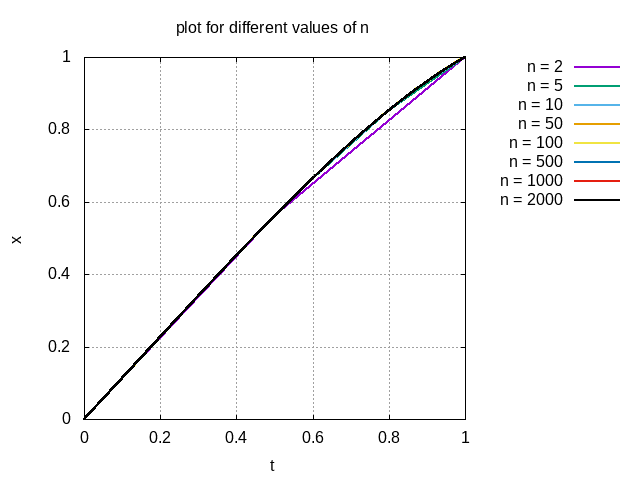
\includegraphics[scale=0.7]{Plots/plot_x(t).png}
        \end{center}
        The curves are overlapping because the points obtained for different values of n had very same value up to 4 to 5 decimal places. For n = 2 the curve can be distinguished and for n = 5 the curve is almost overlapping and curves of n = 10, 50, 100, 500, 1000, 2000 are completely overlapping.\\
    	\begin{center}
            \begin{tabular}{cc}
                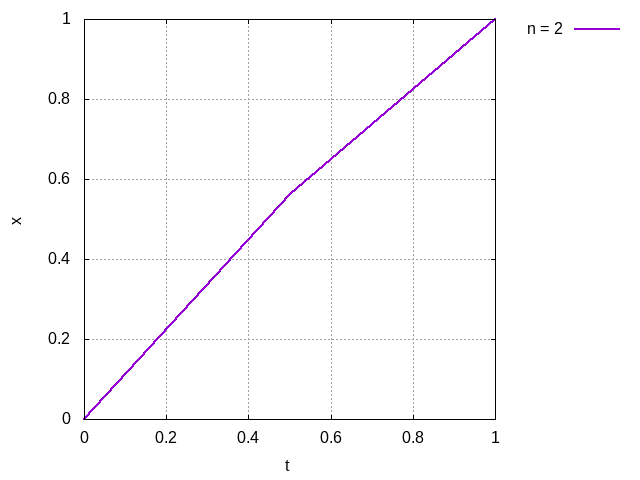
\includegraphics[scale=0.5]{Plots/plot_n_2.png} & 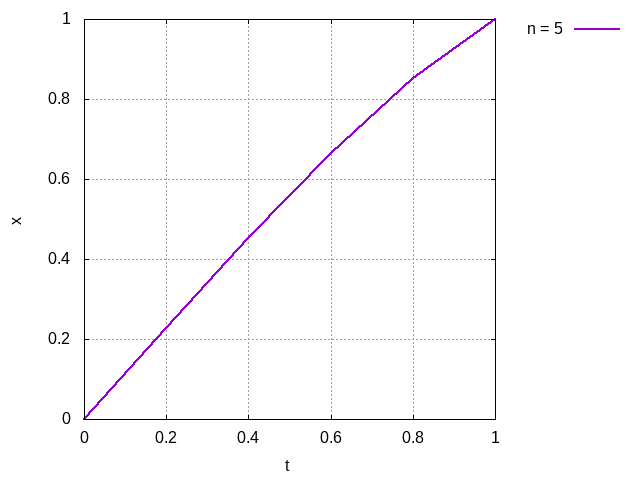
\includegraphics[scale=0.5]{Plots/plot_n_5.png}\\
                (a) & (b)\\
                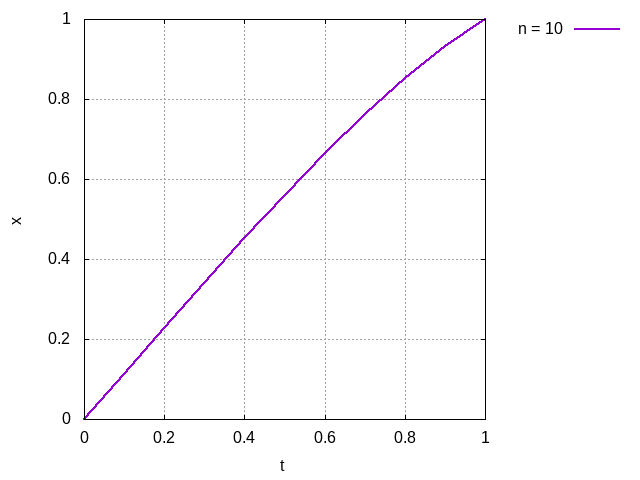
\includegraphics[scale=0.5]{Plots/plot_n_10.png} & 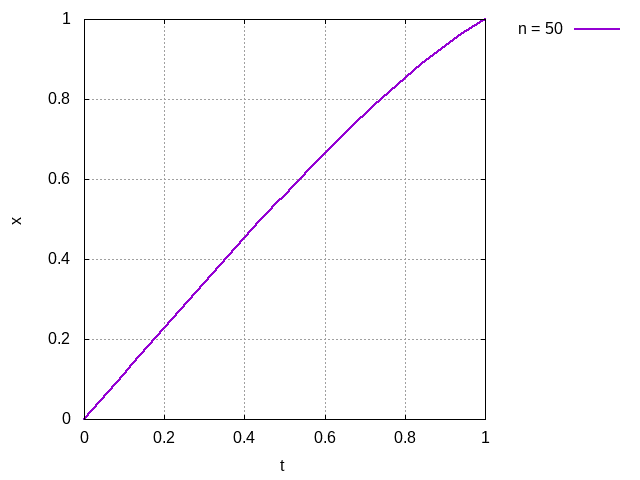
\includegraphics[scale=0.5]{Plots/plot_n_50.png}\\
                (c) & (d)\\
                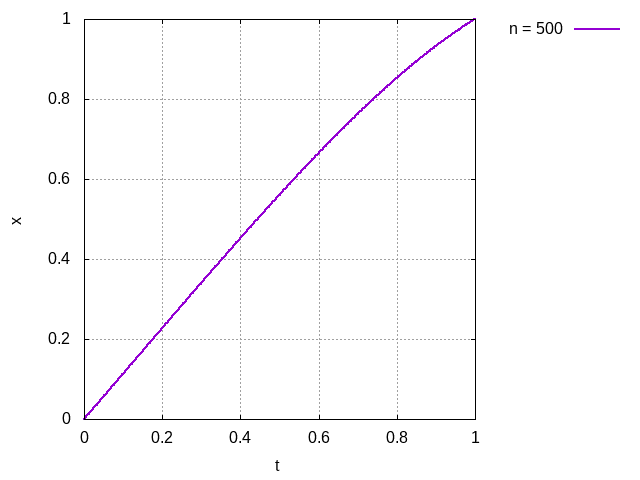
\includegraphics[scale=0.5]{Plots/plot_n_500.png} & 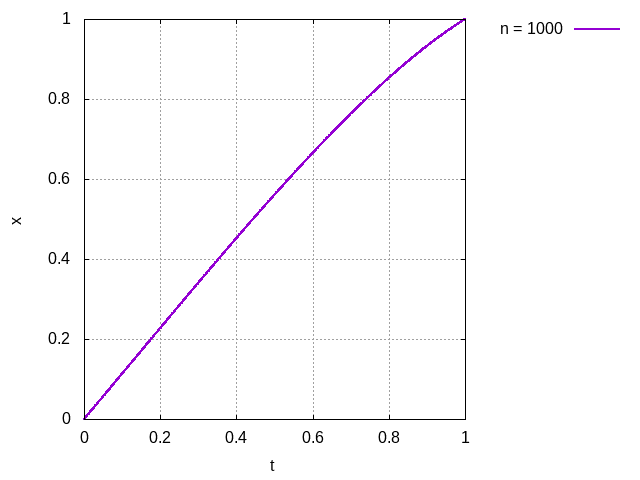
\includegraphics[scale=0.5]{Plots/plot_n_1000.png}\\
                (e) & (f)\\
            \end{tabular}
            \captionof{table}{Graphs for different values of n a) 2; b) 5; c) 10; d) 50; e) 500; f) 1000}
    	\end{center}
    \section{Conclusion}
    \begin{itemize}
        \item The given problem can be solved with 10 intervals.
        \item Time and Space complexity of solving tridiagonal matrix for given problem with gauss elimination is \textbf{O(n)} where n is number of intervals.
    \end{itemize}
\end{document}
